%%% thesis.tex
%%% no more needs to be said
%
% Alex Barnett, Sept 2000.
%
% Taken from Adam Lupu-Sax and edited May 2000.

% my preferred settings:
% \documentclass[11pt,twoside,final]{huthesis}

% Harvard GSAS Jan 2000 settings:
% (Lauren Lamir 5-1519 gave 12pt Times New Roman as the ideal size)...
\documentclass[12pt,oneside,final]{UCOthesis}

\usepackage[utf8]{inputenc}
\usepackage{epsfig,bm,epsf,float}
\usepackage{apacite}
\usepackage{graphicx}
\usepackage{tikz}
\usepackage{amsmath,amsfonts,amssymb,amsthm}
\usepackage{listings}
\usepackage{color}

\setcounter{tocdepth}{2}

% Graphics
\usetikzlibrary{arrows,positioning,shapes} 
\tikzset{
    %Define standard arrow tip
    >=stealth',
    %Define style for boxes
    box/.style={
           rectangle,
           rounded corners,
           draw=black, very thick,
           text width=6.5em,
           minimum height=2em,
           text centered},
    % Define arrow style
    arrow/.style={
           ->,
           thick,
           shorten <=2pt,
           shorten >=2pt,},
    rect/.style={
               rectangle,
               draw=black, very thick,
               text width=6.5em,
               minimum height=2em,
               text centered}
}
\usetikzlibrary{arrows,positioning,shapes} 
\tikzset{
    %Define standard arrow tip
    >=stealth',
    %Define style for boxes
    punkt/.style={
           rectangle,
           rounded corners,
           draw=black, very thick,
           text width=6.5em,
           minimum height=2em,
           text centered},
    % Define arrow style
    pil/.style={
           ->,
           thick,
           shorten <=2pt,
           shorten >=2pt,}
}

\begin{document}

% Front Matter %
%% frontmatter.tex
%%

\titulo{Compilador Imperativo-Funcional}
\autorA{Juan Felipe Cañizares Corrales}
\autorB{Lukas Restrepo Suarez}
\degreemonth{Julio} % month final submission occurs.
\degreeyear{2015}
\facultad{factultad de ingeniería}
\programa{ingeniería de sistemas}
\titulooptar{ingeniero de sistemas}
\asesorA{Daniel Cañizares Corrales}
\asesorB{Mario Zuluaga Tobón}

\fecha{21/04/2015}
\ciudad{Rionegro}

\maketitle
\copyrightpage
\entregapage




%We show how a systematic subtraction of the `special' components of a general
%deformation can be used to give an improved
%version of the `wall formula' estimate for $\mu(0)$.
%We believe this is the first study of $\omega$-dependent heating rate in
%billards, and the first consideration of the `special' nature of dilation.



% these are optional in the Jan 2000 Harvard thesis GSAS guide:
%\listoffigures
%\listoftables
%(Cut them for my personal thesis format).



% Dedicatoria %
\begin{dedication}
	\begin{quote}
		\hsp
		\em
		\raggedleft
		
		Dedicado a las List of Comprehension,\\
		sin ellas este trabajo\\
		no hubiera sido posible.
		
	\end{quote}
\end{dedication}

% Agradecimiento %
\begin{acknowledgments}


\end{acknowledgments}

% Tabla de contenido %
\addcontentsline{toc}{section}{Tabla de Contenido}
\tableofcontents

\newpage

% Abstract - Resumen %
\begin{abstract}

\end{abstract}

\startarabicpagination

%%% end



% Marco teórico %
\part{Marco Teórico}
%% Marco Teórico C1 %%

\chapter{Paradigmas}

``Las herramientas que utilizamos tienen una profunda (¡y retorcida!) influencia en nuestros hábitos de pensamiento, y, por lo tanto, en nuestra habilidad mental'', Edsger Dijkstra. \\

Los paradigmas de programación son modelos que guían la forma en que debemos pensar para resolver problemas utilizando herramientas computacionales. Cada paradigma tiene sus ventajas y desventajas de acuerdo al tipo de problema que se deseé resolver. En este capítulo revisaremos los dos principales modelos que soportan las corrientes  \emph{imperativa} y \emph{funcional}.

\section{Modelo computacional}



\subsection{Máquina de Turing}

\subsection{Cálculo Lambda}

El cálculo lambda $\Lambda$ desarrollado por Alonso Church en los 30 para dar una teoría general de las funciones. Tiene por objeto formalizar el empleo de funciones como transformación de argumentos en resultados empleando 
un conjunto de axiomas, y reglas de inferencia.

\subsubsection{Sintaxis}

Dado un conjunto \texttt{A} de nombres de variables tal que $\vert$ 
\texttt{A} $\vert = \mathbb{N}$, una expresión lambda \texttt{<expr>} es una produccion de FNB ``Forma normal de Backus $\mathfrak{F}$":

\begin{verbatim}
<expr> ::= <variable> 
        |  <variable>.<expr> 
        |  (<expr><expr>)
\end{verbatim}

\begin{note}
Para denotar términos usamos letras mayúsculas \texttt{M,N, $\dots$} y para denotar variables letras  minúsculas \texttt{$x,y, \dots$}
\end{note}

Una abstracción funcional crea procedimientos y funciones y los invocara mediante un nombre donde se destaca qué hace la función y se ignora cómo lo hace, está será:

\texttt{$\lambda$<variable>.<expr>}
donde:
\texttt{$\lambda$<variable>} es la lista de argumentos
\texttt{<expr>} es el contenido de la abstracción funcional

Una función con más de un argumento se representará:
\texttt{$\lambda $x$_1. $x$_2. \dots $x$_n. $M}

\begin{defn}[Equivalencia entre expresiones de $\Lambda$]\end{defn}

Aplicación funcional  \texttt{(M N)} la cual produce un resultado \texttt{R} la consistencia implica una interpretacion equivalente,
es decir \texttt{(M N)} $\equiv$ \texttt{R}, luego representan lo mismo.
El resultado de una aplicación funcional será obtenido mediante la generación de expresiones equivalentes:

\begin{defn}[Relaciones de equivalencia entre expresiones de $\Lambda$]
\end{defn}
\begin{itemize}
\item Reflexividad: \texttt{M $\equiv$ M}
\item Simetría: \texttt{M $\equiv$ N $\Rightarrow$ N $\equiv$ M}
\item Transitividad: \texttt{M $\equiv$ N $\wedge$ N $\equiv$ P $\Rightarrow$  M $\equiv$ P}
\item \texttt{M $\equiv$ N $\Rightarrow$ (M P) $\equiv$ (N P)}
\item \texttt{M $\equiv$ N $\Rightarrow$ (P M) $\equiv$ (P N)}
\item \texttt{M $\equiv$ N $\Rightarrow$ $\lambda$x.N $\equiv$ $\lambda$x.M}
\end{itemize}

\begin{defn}[Ocurrencia $\succ$ de un $\lambda$-termino]\end{defn}
\begin{itemize}
\item \texttt{$\succ$P $\in$ P}
\item \texttt{$\succ$P $\in$ M $\vee$ N $\Rightarrow \ \succ$P $\in$ (M N)}
\item \texttt{$\succ$P $\in$ M $\vee$ P $\equiv$ x $\Rightarrow \ \succ$P $\in$ ($\lambda$x.M)}
\end{itemize}

\begin{defn}[Ocurrencia $\succ$ de un $\lambda$-variable ligada \texttt{b} o libre \texttt{f}]\end{defn}
Una ocurrencia de la variable \texttt{b} en un término \texttt{P} es ligada sí y solo sí, \texttt{b} ocurre en un subtérmino de \texttt{P} de la forma \texttt{$\lambda$b.M} es decir 
\texttt{Q $\subset $ P $ := \lambda$b.M
$\Rightarrow \ \succ$b $\in$ P $\Leftrightarrow$ 
$\succ$x $\in$ Q}. \\
La ocurrencia es libre cuando \\
\texttt{$\succ$f $\in$ N $ := \lambda$z.M $\wedge$
f$\neq$z 
$\Rightarrow \ \succ$f $\in$ N $\Leftrightarrow  
$ f $\equiv$ N $\vee \ \succ$f $\in$ M }


\begin{defn}[Reglas de reduccion]\end{defn}
\begin{itemize}
\item $\beta$-reducción
\item $\alpha$-reducción
\item $\eta$-reducción
\end{itemize}

\section{Lenguajes de programación}

\subsection{Imperativo}

\subsection{Declarativo}
%% Marco Teórico C2 %%

\chapter{Teoría Funcional}

Llamamos programación funcional a un paradigma, el cual comenzó a principios de los sesenta, impulsado por la necesidades de los científicos de la inteligencia artificial, y que cubriera los procesos del cálculo simbólico, teoría de pruebas, pruebas de teoremas, en tal época ningún lenguaje imperativo daba una aproximación a estas necesidades.\\
La programación funcional trata los cálculos como funciones matemáticas, no hay la noción de posición de memoria, por tanto tampoco asignación, a través de la aplicación de los teoremas de recursividad se operan los bucles, también se distingue la notación frente a lenguajes imperativos clásicos. Hoy en día, algunos lenguajes de programación han tratados de implementar este paradigma.\\
La programación funcional se cimenta en el cálculo lambda desarrollado por Church en los treinta para dar una teoría paralela de funciones, este provee a la programación de sintaxis, semántica para definir función y permite definir primitivas de programación.\\
En la actualidad los lenguajes funcionales son Haskell, Scheme, Erlang, Rust, OCaml, el interés principal de la programación funcional es académico, aunque a veces se usa en la industria en ciertos desarrollos, por ejemplo con F#.

%% Marco Teórico C3 %%

\chapter{Compiladores}

\section{Historia}

\section{Interprete}
	\subsection{Compilador}
	\subsection{Interprete}

\section{Lenguajes formales}

\section{Partes de un compilador}

	\subsection{Front-End}
	\subsection{Middle-End}
	\subsection{Back-End}

\section{Construcción de un compilador}





% Capítulos %
\part{Capítulos}
%% intro.tex

\chapter{Introduction and summary}
%%%%%%%%%%%%%%%%%%%%%%%%%%%%%%%%%%%%%%%%%%%%%%%%

\subsubsection{Structure of this thesis}

\cite{art1}
This thesis falls naturally into four parts, which are relatively
independent:
\begin{itemize}
\item Study of dissipation rate in deformed chaotic billiards (Chapters~2,
3 and 4),
\item Improved numerical methods for quantization of billiards
(Chapters~\ref{ch:ipwdm} and \ref{ch:verg}),
\item Half-plane scattering
%theory
approach to mesoscopic conductance
(Chapter~\ref{ch:qpc}), and
\item Design of an atom waveguide using two-color evanescent light fields
(Chapter~\ref{ch:atom}).
\end{itemize}

The first two parts form the main body of the thesis, and they are both
devoted to the study of billiard systems (hard-walled cavities
enclosing a region of free space)
in which the classical motion is chaotic.
The quantum mechanics of such systems has become known as the field of
`quantum chaos'.
The first part probably contains the most significant new physical results;
this is reflected in the choice of thesis title.
The second part can be viewed merely as a description of numerical
quantum-mechanical calculations that play a
supporting role in the first part.
However, there will also turn out to be a surprising reciprocal connection,
namely that results from the first part will provide a much-needed
explanation for the success of a very efficient numerical technique
in the second part.
The intertwining of these two subject areas had turned out to be one of the
most beautiful surprises in this body of research.

The third and fourth parts form essentially separate projects, and can
therefore be read independently.
However they do share with the rest of the thesis the common theme of
wave mechanics: the third presents a new approach to
the transport of quasiparticle waves in mesoscopic systems,
and the fourth models confined electromagnetic waves to trap and guide atoms
(which themselves can be treated as coherent matter waves).

The goals and subject matter of the four parts are sufficiently different
to merit individual introductions and summaries, which now follow without
further ado.



% 1111111111111111111111111111111111111111111111111111111111111111111111111111
\subsubsection{Chapters 2,3 and 4: Dissipation rate and
deformations of chaotic billiards}


The dynamics of a particle inside a cavity
(billiard) in $d=2$ or 3 dimensions 
is a major theme in studies of classical and quantum chaos
\cite{ottbook,hellerleshouches,berryleshouches}.
Whereas the physics of time-independent chaotic systems 
is extensively explored, less is known 
about the physics when such a system is `driven' (time-dependent
chaotic Hamiltonian).
The main exceptions are the studies of 
the kicked rotator and related systems \cite{qkr}. 
However, the rotator (with no kicks) 
is a $d=1$ integrable system, whereas we 
are interested in chaotic ($d\ge2$) cavities.


Driven cavities have been of special interest since the 1970s in
studies of the so-called `one-body' dissipation rate in vibrating nuclei 
\cite{wall,koonincl,kooninqm,jarz92,jarz93}.
A renewed interest in this problem is anticipated
in the field of mesoscopic physics. Quantum dots \cite{been,dittrich}
can be regarded as small 2D cavities whose shape 
is controlled by electrical gates. Quasiparticle motion inside the dot
can have long coherence (dephasing) times,
and enable the semiclassical regime to be approached (many wavelengths
across the system).


In Chapter~\ref{ch:review} I give tutorial review of the
theory of dissipation in general driven
ergodic systems, which is quite a young field.
The Hamiltonian is controlled by a single parameter $x$, whose
time-dependence will be $x(t)=A\sin(\omega t)$ where $A$ is the amplitude  
and $\omega$ is the driving frequency.
In both the classical (Section~\ref{sec:classreview}) and quantum-mechanical
(Section~\ref{sec:qmreview}) pictures, dissipation is a result of
{\em stochastic energy spreading}.
Once this spreading is established, the pictures can be unified \cite{doronfrc}.
Irreversible growth of energy (heating) is then a result of biased diffusion
(a random walk) in energy.
I will confine myself to a regime where linear response theory (LRT) is valid.
In the quantum case this is known as the Kubo formalism, although the
language of the energy spreading picture appears different (I connect the
two pictures in Section~\ref{sec:resp}).
The heating rate is given by

%% intro.tex

\chapter{Parser Combinators}
%%%%%%%%%%%%%%%%%%%%%%%%%%%%%%%%%%%%%%%%%%%%%%%%




%% intro.tex

\chapter{Universo imperativo}
%%%%%%%%%%%%%%%%%%%%%%%%%%%%%%%%%%%%%%%%%%%%%%%%

Existen dos grandes modelos computacionales: el funcional, basado en el calculo lambda de Alonzo Church, y el imperativo, basado en la máquina de Turing, inventada por Alan Turing. La exploración de estos modelos no sólo hace parte de la teoría computacional, sino también, de lenguajes formales y compiladores, pues cada modelo de cómputo genera diferentes paradigmas que definen el lenguaje y su implementación.

\paragraph{El modelo computacional es indiferente,} tal como lo plante la tesis Church-Turing (CT)\footnote{La tesis CT no es un teorema.}, una máquina de Turing puede simular cualquier otro modelo computacional con máximo una ralentización polinomial, esto tiene como resultado que dada la clase de complejidad \textbf{P}  en el modelo análogo\footnote{Clase de complejidad P, conjunto de problemas solucionables en tiempo polinomial por una máquina determinista.}, esta no es más grande que en una máquina de Turing. Si la tesis es cierta, implicaría que la clase \textbf{P} definida por los alienígenas es igual a la nuestra. \cite{Arora2009}




\section{Funcional vs Imperativo}

Comúnmente tenemos la pre-concepción de que el universo Funcional es excluyente al Imperativo, en cierto sentido puede ser cierto, pues están basados en diferentes modelos computacionales, asumiendo que la tesis CT es cierta, sabemos que todo el conjunto de los problemas solucionables en cualquier modelo computacional determinista (válido) pueden ser solucionados con los dos enfoques, es decir, ambos modelos son igualmente poderosos, la pregunta que se podría hacer es, ¿existe alguna manera de comunicar ambos universos para aplicar técnicas existentes que solo se encuentran en alguno de los dos?

Actualmente todos los lenguajes de programación modernos mezclan atributos de ambos paradigmas creando a su vez nuevos paradigmas que dotan a los lenguajes de gran flexibilidad. Según \textsc{Beckman}, en el inicio de la computación moderna, el mundo se partió en dos campos, el campo \emph{bottom-up} teniendo como base las máquinas de Turing, empezando con el hardware y añadiendo abstracción a medida que sea necesario, cada vez acercándose mas a las matemáticas pero nunca perjudicando el performance, el otro campo \emph{top-down} parte de las matemáticas y cada vez quita abstracción para acercarse a la máquina sin importar el performance, comenzando desde el calculo lambda, actualmente se está llegando a un punto de equilibrio entre ambos campos \cite{Beckman2007}  . Esto es posible con la definición de un lenguaje que permita utilizar estructuras pertenecientes a cada uno de los enfoques computacionales, esto puede responder en cierta medida la pregunta anterior, pero ¿que sucede si el lenguaje no soporta todas las estructuras necesarias para realizar distintas técnicas que solo pertenecen a un enfoque?\\

La implementación de un lenguaje funcional en una máquina imperativa requiere de múltiples transformaciones y optimizaciones de bajo nivel, esto permite crear lenguajes funcionales con un desempeño aceptable, de no ser así, como resultado se tendría un lenguaje funcional con grandes fallas de desempeño.

Los compiladores más eficientes están escritos en C++, lenguaje multiparadigma (mayormente imperativo), que permite una buena capacidad de abstracción y no es lejano a la máquina, por lo cuál, en términos de performance, éste lenguaje es el más apropiado. El problema radica en que el universo funcional, es más cercano al problema de los compiladores, fácilmente se puede entender la anterior afirmación con la implementación de un front-end, el cuál es declarativo, son múltiples funciones interactuando, que retornan estructuras y realmente no importa mucho el concepto de estamento, la generación de estructuras recurrentes y pattern matching en lugar de estructuras complejas con punteros y switches.

Luego, no quiere decir que acercarse con un enfoque imperativo suponga una aproximación errada, mas bien, reduce la expresividad en el dominio del problema.\\

Una solución plausible podria ser crear un nuevo lenguaje $L^*$ que soporte ambos paradigmas, partiendo de éste escribir un compilador con las técnicas funcionales sin perder mucho performance, pero escribir el compilador para el lenguje $L^*$ sería demasiado complejo.



	\subsection{Arquitectura Von-Neumann}
	La popularidad del modelo imperativo se debe a la arquitectura del computador que usamos, la arquitectura Von-Neumann, inventada por el matemático Húngaro-Estadounidense con el mismo nombre. Es fácil notar que aunque la máquina de Turing y el cálculo lambda son altamente abstractos, el primero está mucho mas cerca a una implementación real de un computador basado en la tecnología digital. La arquitectura Von-Neumann está más ligada al concepto de estamentos que modifiquen el estado de la máquina, que a la composición de funciones puras.\\\\
	
	\begin{figure}[H]
		\centering
		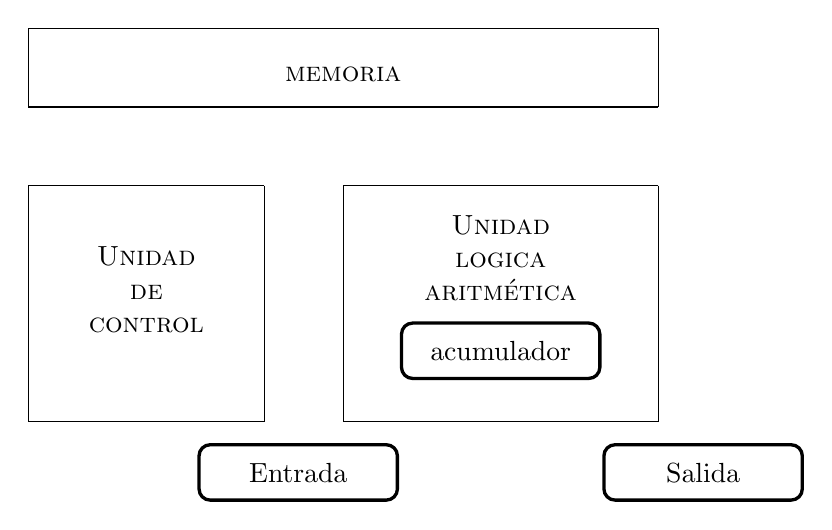
\begin{tikzpicture}
		\coordinate (ma) at (0,0);   
		\coordinate (mb) at (8,0);
		\coordinate (mc) at (8,1);
		\coordinate (md) at (0,1);   
		
		\coordinate (ca) at (0,-1);
		\coordinate (cb) at (3,-1);
		\coordinate (cc) at	(3,-4);
		\coordinate (cd) at (0,-4);
		
		\coordinate (aa) at (4,-1);
		\coordinate (ab) at (8,-1);
		\coordinate (ac) at	(8,-4);
		\coordinate (ad) at (4,-4);		
		
		% Memoria
		\draw (ma) -- (mb) node [above=2mm, midway] {\textsc{memoria}};
		\draw (mb) -- (mc);
		\draw (mc) -- (md);
		\draw (md) -- (ma); 
		
		% Unidad de control
		\draw (ca) -- (cb) node [below=6mm, midway] {\begin{tabular}{c}
			\textsc{Unidad}\\\textsc{de}\\\textsc{control}
		\end{tabular}};
		\draw (cb) -- (cc);
		\draw (cc) -- (cd);
		\draw (cd) -- (ca);
		
		% Memoria
		\draw (aa) -- (ab) node [below=2mm, midway] (ALU) {\begin{tabular}{c}
			\textsc{Unidad}\\\textsc{logica}\\\textsc{aritmética}
		\end{tabular}};
		\draw (ab) -- (ac);
		\draw (ac) -- (ad);
		\draw (ad) -- (aa);    
		
		\node [below=0.1mm of ALU] [box] (ac) {acumulador};
		\node [below left=8mm and 0.1mm of ac] [box] (i) {Entrada};
		\node [below right=8mm and 0.1mm of ac] [box] (o) {Salida};
		
		
		\end{tikzpicture}
		
		\caption{Arquitectura Von-Neumann}
		\label{figram}
	\end{figure}
	
	Todos los computadores digitales están basados en ésta arquitectura; la pregunta que podría surgir es ¿como los computadores pueden ejecutar código funcional?. Partimos de que la solución algorítmica de un problema es distinta en el modelo funcional e imperativo, pero en ambos se puede solucionar el problema. Así pues, si se construyera una máquina basada en una arquitectura funcional, ésta debe entender un lenguaje máquina muy abstracto basado en el cálculo lambda. Llámese $M^f$ a ésta máquina funcional, ésta no debe entender código imperativo, al igual que una máquina imperativa no entiende código funcional, así pues, debe existir una forma de representar el código funcional en imperativo y viceversa partiendo de la \emph{tesis CT}, pues ambos modelos parecen ser análogos.
	
	Lo anterior permite responder a la posibilidad de escribir código funcional en una máquina imperativa, al fin y al cabo, cualquier código terminará siendo código imperativo de bajo nivel entendido por el computador, ésta labor es realizada por el \emph{compilador}. Si careciéramos de la teoría de compiladores no sería plausible la utilización de cualquier tipo de programación funcional. En términos generales, la utilización de la programación funcional en una máquina imperativa no es más que una ilusión, es decir, es sólo la expresividad del lenguaje, pues el compilador es el encargado de transformar de alguna forma dicho código a una representación imperativa.
	
	Resulta bastante difuso lograr separar y representar los dos modelos computacionales desde éste punto, tan sólo se puede afirmar que uno esta basado en la máquina de Turing y el otro en el cálculo lambda, y dado que una solución en un modelo puede ser reducida o representada como el otro, se puede reafirmar su naturaleza análoga. Pero más allá de ésto es difícil definir la interacción y estructura de cada uno, partiendo desde los compiladores sólo podrían definirse como paradigmas, que incluso se pueden mezclar en un lenguaje pues al final serán traducidos a una representación genérica. 
	
	
\section{Parser imperativo clásico}
El análisis sintáctico o parsing está presente en todos los compiladores, puesto que es la fase que se encarga de evaluar el programa fuente verificando que éste cumpla con las especificaciones del lenguaje definido para el compilador \cite{MarioZ}, ademas, realiza la representación intermedia que será utilizada por el \emph{back-end} para optimizar y generar código \cite{Dragon}.

Existen múltiples formas de diseñar un parser, pero la más común es la forma \emph{descendente}, puede verse como el problema de construir un árbol de análisis sintáctico para la cadena de entrada, partiendo desde la raíz y creando los nodos del árbol de análisis sintáctico en preorden.\cite{Dragon}

Así pues, si se quisiera construir un parser descendente por la izquierda se deben crear tantas funciones como no terminales existan, y en cada una se verifica si la estructura interna de la regla es correcta o no.

\begin{exmp}
	Sea $G_1$ una gramática válida sobre el lenguaje $L'$, y $G_1 \in LL(1)$.
	Donde $G_1$ está definido por:
		
	\begin{lstlisting}
	FUNCTION -> 'function' '(' PARAMS ')'
	PARAMS   ->  var ',' PARAMS | E
	\end{lstlisting}
	
	$G_1$ no es una gramática recursiva por la izquierda y tampoco es ambigua.
	
	Así se construirá un parser descendente por la izquierda imperativo clásico:
	\begin{lstlisting}[language=C++, caption="Parser imperativo"]
	void FUNCTION()
	{
		if(current_token == token.function){
			if(current_token == '('){
				PARAMS();
				if(current_token != ')')
					cout << "ERROR\n";
			}
			else
				cout << "ERROR\n";
		}
		else{
			cout << "ERROR\n";
		}
	}
	
	void PARAMS()
	{
		if(current_token == token.var){
			if(current_token == ','){
				PARAMS();
			}
		}
	}
	\end{lstlisting}
\end{exmp}

	Como se puede observar un parser imperativo clásico se vuelve rápidamente inmanejable, por ésta razón existen generadores de analizadores sintácticos, pero éstos últimos tienen un gran problema, que generan una enorme cantidad de código a espaldas del programador.
	
	A simple vista se puede observar la gran desventaja que tiene esta forma de implementar los analizadores sintácticos, están totalmente desligados de la gramática, y teniendo en cuenta que aún no se han implementado las estructuras para crear el árbol de sintaxis abstracta, omitiendo el análisis léxico y la definición de los tokens y la demás estructura presente en la clase que contiene el parser.


\section{Parser Funcional sobre un lenguaje imperativo}

La necesidad de crear un parser elegante y sencillo en el universo imperativo es obvia. Ya se ha descrito los componentes esenciales y los recursos que debe proveer el lenguaje para que los \emph{Parser Combinators} puedan ser implementados. Al comprar el parser imperativo con el funcional se encuentra una abismal diferencia, y marcan como claro ganador a los  \emph{Parser Combinators}. Partiendo de los mecanismos de abstracción de \emph{C++} descritos en el primer capítulo se podría desarrollar una librería básica que intente simular los ya mencionados parsers funcionales.

	\subsection{Tipo del parser}
	Tal como se han implementado los \emph{Parser Combinators} en \emph{Haskell}, es menester definir el tipo del parser, y en el mundo imperativo continua siendo igual de importante éste primer paso.
	
	\begin{lstlisting}[language=C++, caption="Tipo Parser"]
	template<typename R>
	struct Parser{
		vector<pair<R,string>* > result;		
	};
	\end{lstlisting}

	La definición del tipo del parser cumple con los mismos objetivos que la definida en el universo funcional. El template permite simular el polimorfísmo presente en los parsers funcionales implementados en \emph{Haskell}, así pues, el resultado del mismo puede ser cualquier tipo de dato definido para el análisis sintáctico. 
	Se puede notar que la definición que se ha utilizado es la simplificada por \textsc{Hutton}, en la cuál la entrada es siempre un \emph{string}, obviamente puede ser remplazado por un argumento en el template lo que dotará de mayor flexibilidad al parser para que pueda recibir cualquier tipo de dato.
	
	El atributo \texttt{result} cumple la función de lista de éxito (\emph{Success list}), dicha lista está implementado con un \texttt{vector} de \texttt{pair}, es decir, una lista de pares ordenados, donde cada par cumple con la misma definición dada en el capítulo 2.
	
	\subsection{Creación de un Parsers básicos}
	Al igual que en \emph{Haskell} es necesario la creación de los parsers elementales que permitirán implementar parsers mucho más complejos con el fin de evaluar una gramática.
	
	Los tres parsers básicos son:
	\begin{itemize}
		\item Symbol: Reconoce un símbolo.
		\item Succeded: Tiene éxito sin consumir ningún caracter de entrada.
		\item Fail: Falla siempre sin consumir ningún caracter de entrada.
	\end{itemize}
	
	La implementación de estos parsers en \emph{C++} es un poco más tediosa y menos clara que en \emph{Haskell}.
	
	\begin{lstlisting}[language=C++, caption="Parsers básicos"]
		template <char t>
		Parser<char> symbol (string xs)
		{
			Parser<char> parser;
			auto x = xs.back() == t;
			if (x)
			{
				xs.pop_back();
				pair<char,string>* result = new pair<char,string>(t,xs);
				parser.result.push_back(result);
			}			
			return parser;
		}
		
		template<char t>
		Parser<char> succeded(string xs)
		{
			Parser<char> parser;
			parser.result.push_back(new pair<char,string>(t,xs));
			return parser;
		}
		
		template<char t>
		Parser<char> fail(string xs)
		{
			Parser<char> parser;
			return parser;
		}		
	\end{lstlisting}
	
	Todos los anteriores métodos retornan un parser: \texttt{Parser<char>}, es decir, que el resultado del análisis será un caracter, al igual que la definición en el modelo análogo ya mencionado.
	
	La utilización de estos parsers es muy simple, solo hace falta tener un string de entrada, y en el caso de \emph{symbol} un símbolo (caracter) para hacer el reconocimiento.
	
	\begin{lstlisting}[language=C++]
	Parser<char> P = symbol<t>("otxet"); //C++
	symbol 't' "texto"					//Haskell
	\end{lstlisting}
	En comparación con la utilización del mismo parser en \emph{Haskell}, se mantiene la similitud.
	
	A la hora de utilizar los parsers aquí descritos, es necesario reversar el string de entrada, esto por motivos de optimizaciones, pues la definición de eliminar la primera posición de un string en \emph{C++} es $\Theta$(n), por el contrario, eliminar la última posición se logra en tiempo constante $\Theta$(1).
	
	\subsection{Currying imperativo}
	Como se expuso en el capítulo anterior, el currying es un elemento básico en los \emph{Parser Combinators}, y sobretodo en la definición de los mismos desde un punto totalmente teórico. La currificación en el mundo funcional provee gran flexibilidad, especialmente si de la \emph{evaluación parcial de funciones} se trata. La evaluación parcial de funciones es precisamente lo que permite inyectar \emph{funciones semánticas} a través de cada resultado de los parsers.
	Es necesario crear un mecanismo de currying en \emph{C++} para poder implementar \emph{Parser Combinators} fieles a la teoría funcional.
	
	\begin{exmp}
		Sea la función $f$ de tipo
		$f:(X \times Y) \to Z$ es igual a a lu función currificada que crea la siguiente función \texttt{curry}$(f): X \to (Y \to Z)$, en otras palabras, cualquier función con múltiples parámetros puede ser expresada como una secuencia de funciones que toman un parámetro.		
	\end{exmp}
	
	En \emph{C++} no existe un currying automático como en \emph{Haskell}, sin embargo, se pueden simular por medio de las expresiones lambda.
	
	\begin{exmp}
		Sea la función $g(x,y) = y$, puede expresarse como \texttt{curry}$(g): x \to (y \to y)$, donde $x$ y $y \in \Z$ . En \emph{Haskell} se puede realizar de forma trivial:
		\begin{lstlisting}[language=Haskell, caption=g currificada en Haskell]
		g	::	Int -> Int -> Int
		g x y = y
		\end{lstlisting}
		
		En \emph{C++} es más complejo pues se debe expresar explícitamente la función currificada.		
		
		\begin{lstlisting}[language=C++, caption=g currificada en C++]
		auto g = [](int x){ return [](int y) { return y; }; };
		\end{lstlisting}	
		
		De ésta manera, se puede evaluar parcialmente la función $g$, es decir, si a g se le envía el parámetro $x$, se obtendrá como resultado otra función que esperará el parámetro $y$.	
	\end{exmp}
	
	\subsection{Varadic templates}
	Diseñar una librería en un lenguaje imperativo partiendo de la teoría funcional es un problema para nada trivial. Múltiples soluciones pueden existir para lograr traducir la expresividad de alto nivel de un lenguaje funcional a un lenguaje imperativo; la mayor complicación radica en que un lenguaje como \emph{C++} no posee la enorme cantidad de mecanismos heredados del \emph{calculo lambda}, si bien \emph{C++} soporta muchísimos más que los lenguajes imperativos promedio, se deben diseñar mecanismos que simulen los presentes en el lenguaje funcional. 

	Las funciones más complejas en la implementación de la librería vista en el capítulo 2 son las de los \emph{Parser Combinators}, y en el universo imperativo es mucho más complejo su diseño.
	
	La siguiente implementación ha sido el resultado de un arduo diseño y estudio de la naturaleza misma de los \emph{Parser Combinators}. En el universo imperativo es poco plausible utilizar una función que permita inyectar una \emph{función semántica}, así pues, se ha decidido que la función $<*>$ reciba también la \emph{función semántica currificada}.
	
	\begin{lstlisting}[language=C++, caption=función secuenciadora en C++]
	
	template<typename R, typename F, typename P, typename P2>
	Parser<R> seq (string input, F f, P p, P2 p2)
	{
		auto r = p(input);
		auto r2 = p2(r.result[0]->second);
		/* APLICAR f */
		return f(/* */);
	}	
	\end{lstlisting}
	
	La anterior definición tiene un claro problema, no hay una forma simple de aplicar la función semántica, ademas, para utilizar la función seq se deben llamar tantas veces como parsers existan, lo que generará un anidamiento innecesario de la función, esto se debe a que en \emph{C++} no se pueden crear operadores con un orden jerárquico definido.
	
	Los \emph{Varadic Templates} permiten recibir un número indefinido de parámetros con tipos no definidos, de ésta manera es posible crear una única función secuenciadora que reciba todos los parsers y se encargue de utilizarlos uno a uno.
	
	\begin{lstlisting}[language=C++, caption=función secuenciadora en C++]
	
	template<typename R, typename F, typename P>
	Parser<R> seq (string input, F f, P p)
	{
		auto r = p(input);
		if(r.result.size() == 0){
			Parser<R> r1;
			return r1;
		}		
		auto f1 = f(r);
		return f1;
	}
	
	template<typename R, typename F, typename P, typename... Args>
	Parser<R> seq (string input, F f, P p, Args... args)
	{
		auto r = p(input);
		if(r.result.size() == 0){
			Parser<R> r1;
			return r1;
		}
		auto f1 = f(r);
		return seq<R>(r.result[0]->second, f1, args... );
	}	
	\end{lstlisting}
	
	De ésta manera es posible crear una función lo suficientemente poderosa y simple que simule los \emph{combinators} de parsers en el mundo funcional. Se recibe la entrada, la \emph{función semántica} y los n parsers que se secuenciarán. Ademas, si un parser falla, se debe retornar una \emph{lista singleton} tal como ocurre en la implementación en \emph{Haskell}.
	
	Esta elegante solución permite sequenciar todos los tipos de parsers que se deseen, e inyecta una \emph{función semántica} permitiendo modificar el retorno de los parsers.
	
	\subsection{$<|>$ imperativo}
	Al igual que en la implementación en \emph{Haskell}, el operador $<|>$ es el más sencillo de todos, y puede ser implementado de forma sencilla de la siguiente manera:
	\begin{lstlisting}[language=C++, caption=función de elección en C++]
	
	template<typename P>
	void or (P& p1, P& p2)
	{
		p1.result.push_back(p2.result[0]);
	}	
	\end{lstlisting}
		
	Ésta función, también puede ser mejorada \emph{sobrecargando} el operador $<|>$, lo que permitiría usarla como si se tratara de un operador \emph{infix} en \emph{Haskell}.
	
	\subsection{Utilización del Parser Combinator Pseudo-Funcional}
	La utilización de los \emph{Parser Combinators Pseudo-Funcionales} se reduce a crear la función semántica y utilizar los \emph{combinators} \texttt{seq} y \texttt{or}. De ésta manera se logran crear parsers que surjan directamente de la gramática.
	
	\begin{exmp}
		Sea $G_1$ una gramática válida sobre el lenguaje $L'$, y $G_1 \in LL(1)$.
		Donde $G_1$ está definido por:
		
		\begin{lstlisting}
		S -> '(' S ')' | e
		\end{lstlisting}
		
		$G_1$ no es una gramática recursiva por la izquierda y tampoco es ambigua.
		La salida del parser debe ser un string que represente los parentesis de la siguiente manera:
		\begin{itemize}
			\item El string ``Inside" representa un parentesis que abre y uno que cierra.
			\item El string ``Empty" representa el caracter $\epsilon$.
		\end{itemize}
		Esto es, si el string de entrada es ``()" la representación del parser deberá ser igual a ``Inside Empty".		
	\end{exmp}
	
	Implementar un parser imperativo clásico para la anterior gramática es simple pero como ya se ha dicho antes supone alejarse totalmente de la gramática, lo que genera un código ilegible.

	La utilización de la librería que se acaba de crear cambia totalmente la perspectiva de la implementación de un parser en el universo imperativo.
	
	\begin{lstlisting}[language=C++, caption=utilización de los Parser combinators en C++]
	Parser<string> parenthesis(string input)
	{
		auto result = seq<string>(input, /*Funcion semantica*/ , 
									symbol<'('>, parenthesis, symbol<')'>) 
				| seq<string>(input, /*Funcion semantica*/ , succeded<'e'>);
		return result;
	}		
	\end{lstlisting}
	
	De ésta manera se implementa fácilmente un parser en \emph{C++}, corto y totalmente relacionado con la gramática, como se puede notar, el \emph{Parser Combinator} \texttt{seq} recibe el input y cada uno de los parsers en orden, muy similar a lo que se hace en \emph{Haskell}. Lo único que falta es definir las funciones semánticas que permitirán retornar un \texttt{Parser<string>}. 
	
	\begin{lstlisting}[language=C++, caption=Funciones semánticas en C++]
		auto l = [](Parser<char> a){
					return [](Parser<string> b){
						return [b](Parser<char> c){
							Parser<string> q;
							q.result.push_back(new pair<string,string>
									("Inside " + b.result[0]->first, 
												c.result[0]->second));
							return q;
					};
				};
			};
		
		auto l2 = [](Parser<char> a){
			Parser<string> q;
			q.result.push_back(new pair<string,string>("Empty", 
								a.result[0]->second));
			return q;
		};		
	\end{lstlisting}
	
	Entendiendo el uso de las \emph{funciones semánticas} se pueden implementar de forma trivial. Cabe anotar que éstas funciones se pueden definir dentro de la llamada de la función secuenciadora, pero no es lo correcto, pues debido a que en \emph{C++} se debe implementar el \emph{currying} manualmente, la longitud de éstas funciones crece mucho y no permite visualizar el parser, es decir, si se implementan de forma separada, como se ha hecho, los parsers quedarán con una sintaxis totalmente directa con la gramática, que es lo que se busca en los \emph{Parser Combinators}.
	
	\begin{lstlisting}[language=C++, caption=utilización de los Parser combinators en C++]
	Parser<string> parenthesis(string input)
	{
		auto result = seq<string>(input, l, 
						symbol<'('>, parenthesis, symbol<')'>) 
			| seq<string>(input, l2, succeded<'e'>);
		return result;
	}		
	\end{lstlisting}
	
	El anterior parser cumple con la definición de la gramática. De ésta manera simple y corta se puede escribir cualquier analizador sintáctico recursivo descendente para una gramática LL(1).
	
	Una vez implementado, se puede utilizar este parser cuantas veces se necesite, para la entrada ``(())" generará la salida:
	\begin{lstlisting}
	[(Inside Inside Empty, ""), (Empty, "))(()")]	
	\end{lstlisting}
	
	Puede parecer extraña la segunda salida, pero hay que recordar que por cuestiones de \emph{performance} se han reversado las entradas.
	
El anterior \emph{Parser Combinator} sobre un lenguaje imperativo no es más que un prototipo inicial,diseños no triviales. A partir de éste punto se deja una hipótesis no demostrada, pues requiere de un análisis profundo de la basta teoría de \emph{mónadas} en el paradigma funcional.


\begin{conj}
	monada
\end{conj}




%% intro.tex

\chapter{Monads}
%%%%%%%%%%%%%%%%%%%%%%%%%%%%%%%%%%%%%%%%%%%%%%%%

\section{Parser Combinator basado en Monads}

\section{Monads y el universo imperativo}

\section{Monad-Parser sobre un lenguaje imperativo}



%% intro.tex

\chapter{FrontEnd Imperativo - Funcional}
%%%%%%%%%%%%%%%%%%%%%%%%%%%%%%%%%%%%%%%%%%%%%%%%

\section{Parser imperativo-funcional}

\section{Compilación del lenguaje}

\section{Comparación}



% Bibliografía %
%%% bibliography for thesis.
\nocite{}

{
\renewcommand{\bibname}{Bibliograf\'ia}
\ssp % single-spacing
\bibliography{./Bibliografia/bibs}
}


% Anexos %
%\appendix
%%%% fokker.tex

\chapter{General transformation of the 1D Fokker-Planck equation}
\label{ap:fokker}

In this Appendix, I show how the drift and diffusion terms $\cdots$

% etc

% example figure:

\begin{figure}[t]
%\centerline{\epsfig{figure=fig1.eps,width=5in}}
\caption[Probability density on the surface $\Omega(E,t)$]{
Projecting a probability density on the surface $\Omega(E,t)$
down to $\rho(E,t)$ in the $E-t$ plane,
or across to $\eta(\Omega,t)$ in the $\Omega-t$ plane.
The gradient $g$ is also shown.
}
\label{fig:fokker}
\end{figure}


We assume a one-to-one time-dependent mapping $\Omega = \Omega(E,t)$,
which can be represented as a (fixed) surface in
three-dimensional $(E,t,\Omega)$ space (Fig. \ref{fig:fokker}).
 $\cdots$



 %%%


% insert other appendices here...

\end{document}
